\chapter{\MakeUppercase{Key Findings / Results from the Paper}}
\setcounter{equation}{0}

\noindent\textbf{Attribution:} All experimental results, tables, comparison images, and performance values in this chapter are reproduced from the supplied report's account of Hong and Kim's paper. They are the authors' reported results, not experiments performed by the student. They have not been independently reproduced for this seminar.\cite{bib1}

\section{\MakeUppercase{Evaluation Metrics}}
To rigorously assess the performance and demonstrate the superiority of the proposed NeRF-DA method, three widely recognized metrics were utilized to compare novel synthesized images against ground truth, or reference views. Comparative experiments were conducted against four established models, including the baseline NeRF and the state-of-the-art Deblur-NeRF, ensuring all models were tested under identical hyperparameter conditions for fair comparison.\cite{bib4}

\subsection{\MakeUppercase{Peak Signal-to-Noise Ratio (PSNR)}}
PSNR was employed as a primary objective metric to assess the fidelity of the reconstruction. It quantifies the degree of quality loss that occurred in the reconstructed images, with higher values indicating superior image quality and lower reconstruction error.

\subsection{\MakeUppercase{Structural Similarity Index (SSIM)}}
The SSIM metric was utilized to evaluate the structural similarity between the synthesized and reference images. SSIM is highly valuable as it assesses image similarity based on three critical factors: brightness, contrast, and structure. The metric inherently shows higher values with less blur, providing a robust measure of perceptual quality.

\subsection{\MakeUppercase{Learned Perceptual Image Patch Similarity (LPIPS)}}
LPIPS was implemented to gauge patch-based similarity using deep features as a perceptual metric. This metric is effective for measuring perceptual differences, as it correlates well with human judgment regarding image quality.

\section{\MakeUppercase{Analysis: Real-World vs Synthetic Data}}
Experiments were conducted using the NeRF BlurData dataset, encompassing scenes affected by two distinct types of degradation: camera motion blur and defocus blur. Camera motion blur arises from camera movement, object motion, or varying lighting conditions. Defocus blur occurs when the camera fails to focus accurately or when the lens aperture is wide open, leading to blurred regions due to a shallow depth of field. The datasets included a large amount of manually captured real-world data and synthetic data generated using Blender. Competitors included ActiveNeRF and DP-NeRF.
\\
\begin{table}[htbp]
\centering
\begin{tabular}{c||ccc|ccc}
\hline\hline
& \multicolumn{3}{c|}{Real camera motion blur} & \multicolumn{3}{c}{Real defocus blur} \\
\cline{2-7}
& PSNR$\uparrow$ & SSIM$\uparrow$ & LPIPS$\downarrow$ & PSNR$\uparrow$ & SSIM$\uparrow$ & LPIPS$\downarrow$ \\
\hline
NeRF & 22.69 & 0.6347 & 0.3687 & 22.40 & 0.6661 & 0.2310 \\
ActiveNeRF & 21.87 & 0.5940 & 0.4153 & 21.23 & 0.6099 & 0.3209 \\
Deblur-NeRF & 25.63 & 0.7675 & 0.1820 & 23.46 & 0.7199 & 0.1342 \\
DP-NeRF & \textbf{25.72} & 0.7614 & \textbf{0.1675} & 23.67 & 0.7299 & 0.1269 \\
\hline
NeRF-DA (Proposed) & 25.64 & \textbf{0.7702} & 0.1679 & \textbf{23.96} & \textbf{0.7337} & \textbf{0.1246} \\
\hline\hline
\multicolumn{7}{l}{\footnotesize The best results are shown in bold.}
\end{tabular}
\caption{Quantitative Comparison on Real-World Data (Poorly Aligned, with Lots of Images))}
\end{table}

\begin{figure}[h]
    \centering
    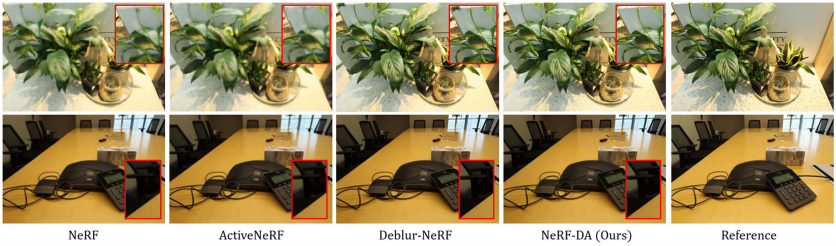
\includegraphics[width=1\linewidth]{Images/realworld.png}
    \caption{Qualitative Comparison on Real-World Camera Motion Blur (Top) and Defocus Blur (Bottom)}
\end{figure}

Quantitative results on real-world data (Table 4.1) for 10 camera motion and 11 defocus scenes revealed that NeRF-DA exhibits top or second-best outcomes across all PSNR, SSIM, and LPIPS metrics when comparing reconstruction to reference views. Significantly, NeRF-DA demonstrated superiority over Deblur-NeRF particularly under camera conditions that were not well aligned with large amounts of images, as evidenced by its stronger SSIM and LPIPS scores. Qualitatively, NeRF-DA consistently produced sharper reconstructions than Deblur-NeRF (Figure 4.1).\cite{bib17}
\\
\begin{table}[htbp]
\centering
\setlength{\tabcolsep}{2.5pt} % Minimal column space
\scriptsize
\begin{tabular}{l|ccc|ccc|ccc|ccc|ccc}
\hline\hline
\textbf{Synthetic} & \multicolumn{3}{c|}{\textbf{Factory}} & \multicolumn{3}{c|}{\textbf{Cozyroom}} & \multicolumn{3}{c|}{\textbf{Pool}} & \multicolumn{3}{c|}{\textbf{Tanabata}} & \multicolumn{3}{c}{\textbf{Trolley}} \\
\cline{2-16}
\textbf{Motion Blur} & P$\uparrow$ & S$\uparrow$ & L$\downarrow$ & P$\uparrow$ & S$\uparrow$ & L$\downarrow$ & P$\uparrow$ & S$\uparrow$ & L$\downarrow$ & P$\uparrow$ & S$\uparrow$ & L$\downarrow$ & P$\uparrow$ & S$\uparrow$ & L$\downarrow$ \\
\hline
NeRF & 19.32 & 0.4563 & 0.5304 & 25.66 & 0.7941 & 0.2288 & 30.45 & 0.8354 & 0.1932 & 22.22 & 0.6807 & 0.3653 & 21.25 & 0.6370 & 0.3633 \\
ActiveNeRF & 18.30 & 0.4131 & 0.5525 & 24.77 & 0.7678 & 0.2388 & 29.13 & 0.7877 & 0.2216 & 21.30 & 0.6487 & 0.3804 & 20.63 & 0.6139 & 0.3941 \\
Deblur-NeRF & \textbf{24.32} & 0.7443 & 0.2717 & 32.24 & 0.9270 & \textbf{0.0441} & 31.56 & 0.8664 & 0.1235 & \textbf{27.09} & \textbf{0.8650} & \textbf{0.1241} & \textbf{27.55} & 0.8655 & 0.1298 \\
\textbf{NeRF-DA} & 24.27 & \textbf{0.7535} & \textbf{0.2648} & \textbf{32.25} & \textbf{0.9276} & 0.0453 & \textbf{31.69} & \textbf{0.8713} & \textbf{0.1132} & 26.11 & 0.8236 & 0.1524 & 27.32 & \textbf{0.8657} & \textbf{0.1230} \\
\hline
\multicolumn{16}{l}{} \\ % Small vertical space

\textbf{Synthetic} & \multicolumn{3}{c|}{\textbf{Factory}} & \multicolumn{3}{c|}{\textbf{Cozyroom}} & \multicolumn{3}{c|}{\textbf{Pool}} & \multicolumn{3}{c|}{\textbf{Tanabata}} & \multicolumn{3}{c}{\textbf{Trolley}} \\
\cline{2-16}
\textbf{Defocus Blur} & P$\uparrow$ & S$\uparrow$ & L$\downarrow$ & P$\uparrow$ & S$\uparrow$ & L$\downarrow$ & P$\uparrow$ & S$\uparrow$ & L$\downarrow$ & P$\uparrow$ & S$\uparrow$ & L$\downarrow$ & P$\uparrow$ & S$\uparrow$ & L$\downarrow$ \\
\hline
NeRF & 25.36 & 0.7847 & 0.2351 & 30.03 & 0.8926 & 0.0885 & 27.77 & 0.7266 & 0.3340 & 23.80 & 0.7811 & 0.2142 & 22.67 & 0.7103 & 0.2799 \\
ActiveNeRF & 24.13 & 0.7643 & 0.2528 & 28.60 & 0.8681 & 0.1093 & 26.36 & 0.6731 & 0.3724 & 22.62 & 0.7477 & 0.2512 & 22.09 & 0.7010 & 0.2892 \\
Deblur-NeRF & \textbf{26.54} & 0.8448 & 0.1362 & \textbf{31.92} & 0.9187 & 0.0456 & 30.64 & 0.8286 & 0.1885 & \textbf{26.19} & \textbf{0.8528} & \textbf{0.0987} & \textbf{25.71} & 0.8201 & 0.1325 \\
\textbf{NeRF-DA} & \textbf{26.54} & \textbf{0.8537} & \textbf{0.1223} & 31.84 & \textbf{0.9188} & \textbf{0.0434} & \textbf{30.71} & \textbf{0.8331} & \textbf{0.1748} & 25.43 & 0.8398 & 0.1209 & 25.45 & \textbf{0.8213} & \textbf{0.1300} \\
\hline\hline
\multicolumn{16}{l}{\tiny The best results are shown in bold.}
\end{tabular}
\caption{Quantitative Comparison on Synthetic Data: Motion Blur (Top) and Defocus Blur (Bottom)}
\end{table}
\begin{figure}[h!]
    \centering
    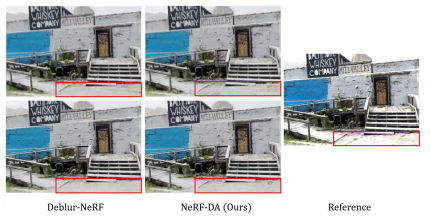
\includegraphics[width=0.8\linewidth]{Images/synthetic.png}
    \caption{Qualitative Comparison on Synthetic Camera Motion Blur (Top) and Synthetic Defocus Blur (Bottom)}
\end{figure}
\newpage
For synthetic data (Table 4.2), NeRF-DA also showed competitive performance. The SSIM scores, which reflect structural quality, confirmed that NeRF-DA consistently surpasses Deblur-NeRF in SSIM scores, except in the Tanabata scene. Furthermore, NeRF-DA proved effective at tackling the issue of data imbalance, which was visually evident in the reduced artifacts on the outer edges compared to Deblur-NeRF, achieving better results overall (Figure 4.2).

\section{\MakeUppercase{Insights from the Ablation Study}}

\begin{table}[htbp]
\centering
\begin{tabular}{l||ccc|ccc}
\hline\hline
& \multicolumn{3}{c|}{Blur Basket} & \multicolumn{3}{c}{Blur Buick} \\
\cline{2-7}
& PSNR$\uparrow$ & SSIM$\uparrow$ & LPIPS$\downarrow$ & PSNR$\uparrow$ & SSIM$\uparrow$ & LPIPS$\downarrow$ \\
\hline
Deblur-NeRF (45 views) & 27.70 & 0.8433 & 0.1395 & 24.63 & 0.7661 & 0.1778 \\
\hline
NeRF-DA (38 views) & 28.29 & 0.8526 & 0.1340 & \textbf{24.73} & \textbf{0.7706} & 0.1678 \\
NeRF-DA (31 views) & \textbf{28.92} & 0.8709 & 0.1071 & 24.54 & 0.7649 & \textbf{0.1593} \\
NeRF-DA (24 views) & 28.90 & \textbf{0.8723} & \textbf{0.1022} & 23.96 & 0.7459 & 0.1751 \\
NeRF-DA (17 views) & 26.44 & 0.8197 & 0.1230 & 23.86 & 0.7477 & 0.1713 \\
\hline\hline
\multicolumn{7}{l}{\footnotesize The result of NeRF-DA training for basket scene while reducing the number of input views.}
\end{tabular}
\caption{Ablation Study: Number of Labeled Images}
\end{table}

The ablation study (the ablation table in this chapter) was conducted to investigate the impact of controlling the number of labeled images extracted from the input blurred dataset. Experiments involved artificially and progressively reducing the holdout test sets from the total multi-view images per scene to evaluate the model's performance under varying data quantity. The results decisively demonstrate that NeRF-DA, trained on an optimal subset of images, outperforms Deblur-NeRF trained on all available views.

This key finding supports the underlying motivation of NeRF-DA, suggesting that the traditional approach of simply incorporating all available views, which includes both view overlap and heavily blurred images, can actually hinder model performance. Conversely, the study also revealed a trade-off: excessively reducing the labeled dataset leads to performance degradation due to insufficient information between surrounding views. Therefore, the optimal number of images for NeRF-DA in each scene is determined by adjusting the data selection based on the light field camera position analysis described in the methods section.
